\documentclass[12pt]{article}
\setlength{\oddsidemargin}{0in}
\setlength{\evensidemargin}{0in}
\setlength{\textwidth}{6.5in}
\setlength{\parindent}{0in}
\setlength{\parskip}{\baselineskip}

\usepackage{amsmath,amsfonts,amssymb}
\usepackage{graphicx}
\usepackage{fancyhdr}
\pagestyle{fancy}


\begin{document}

\lhead{{\bf CSCI 3104 \\ Problem Set 5} }
\rhead{{\bf Instructor\ Buxton \\ Summer 2019, CU-Boulder}}
\renewcommand{\headrulewidth}{0.4pt}

% 60+10+20=90 points possible

\vspace{-3mm}
\begin{enumerate}
    
    % HARD PROBLEM // PROGRAMMING
	\item (60 points) Recall that the \textit{string alignment problem} takes as input two strings $x$ and $y$, composed of symbols $x_{i},y_{j}\in \Sigma$, for a fixed symbol set $\Sigma$, and returns a minimal-cost set of \textit{edit} operations for transforming the string $x$ into string $y$.
	
	Let $x$ contain $n_{x}$ symbols, let $y$ contain $n_{y}$ symbols, and let the set of edit operations be those defined in the lecture (substitution, insertion, and deletion).
	
	Let the cost of \textit{indel} be 1 and the cost of \textit{sub} be 2, except when $x_{i}=y_{j}$, which is a ``no-op'' and has cost 0.
	
	In this problem, we will implement and apply three functions.
	
	(i) {\tt alignStrings(x,y)} takes as input two ASCII strings $x$ and $y$, and runs a dynamic programming algorithm to return the cost matrix $S$, which contains the optimal costs for all the subproblems for aligning these two strings. 
	
	\begin{small}
	\begin{verbatim}
	alignStrings(x,y) :               // x,y are ASCII strings
	   S = table of length nx by ny   // for memoizing the subproblem costs
	   initialize S                   // fill in the basecases
	   for i = 1 to nx
	        for j = 1 to ny
	             S[i,j] = cost(i,j)   // optimal cost for x[0..i] and y[0..j]
	   }}
	   return S
	\end{verbatim}
	\end{small}
	
	(ii) {\tt extractAlignment(S,x,y)} takes as input an optimal cost matrix $S$, strings $x,y$, and returns a vector $a$ that represents an optimal sequence of edit operations to convert $x$ into $y$. This optimal sequence is recovered by finding a path on the implicit DAG of decisions made by {\tt alignStrings} to obtain the value $S[n_{x},n_{y}]$, starting from $S[0,0]$. 
	
	\begin{small}
	\begin{verbatim}
	extractAlignment(S,x,y) :  // S is an optimal cost matrix from alignStrings
	   initialize a            // empty list of edit operations
	   [i,j] = [nx,ny]         // initialize the search for a path to S[0,0]
	   while i > 0 or j > 0
	        a.prepend(determineOptimalOp(S,i,j,x,y)) // what was an optimal choice?
	        [i,j] = updateIndices(S,i,j,a)           // move to next position
	   }
	   return a
	\end{verbatim}
	\end{small}
	
	When storing the sequence of edit operations in $a$, use a special symbol to denote no-ops.
	
	(iii) {\tt commonSubstrings(x,L,a)} which takes as input the ASCII string $x$, an integer $1\leq L \leq n_{x}$, and an optimal sequence $a$ of edits to $x$, which would transform $x$ into $y$. This function returns each of the substrings of length at least $L$ in $x$ that aligns exactly, via a run of no-ops, to a substring in $y$.

	\begin{enumerate}

	\item From scratch, implement the functions {\tt alignStrings}, {\tt extractAlignment}, and {\tt commonSubstrings}. You may not use any library functions that make their implementation trivial. Within your implementation of {\tt extractAlignment}, ties must be broken uniformly at random.
	
	Submit (i) a paragraph for each function that explains how you implemented it (describe how it works and how it uses its data structures), and (ii) your code implementation, with code comments. \label{q:align:code}
	
	Hint: test your code by reproducing the {\tt APE} / {\tt STEP} and the {\tt EXPONENTIAL} / {\tt POLYNOMIAL} examples in the lecture notes (to do this exactly, you'll need to use unit costs instead of the ones given above).
	
	\item Using asymptotic analysis, determine the running time of the call \\ ${}^{}$\hspace{0mm} {\tt commonSubstrings(x, L, extractAlignment(  alignStrings(x,y), x,y  )  )} \\
	Justify your answer.
	
	\item String alignment algorithms can be used to detect changes between different versions of the same document (as in version control systems) or to detect verbatim copying between different documents (as in plagiarism detection systems).
	
	The two {\tt data\_string} files for PS5 (see class Moodle) contain actual documents recently released by two independent organizations. Use your functions from~\eqref{q:align:code} to align the text of these two documents. Present the results of your analysis, including a reporting of 10 of the longest substrings in $x$ of length $L=20$ or more that could have been taken from $y$, and briefly comment on whether these documents could be reasonably considered original works, under CU's academic honesty policy.
		
	\end{enumerate}
	
	\pagebreak
    
	% MEDIUM PROBLEM
	\item (10 points) Shadow is trying to figure out all the potential paths from the bank he is trying to rob to the party's hideout, given by the network below.  Help him calculate the number of paths from node 1 to node 14.
	
	Hint:\ assume a ``path'' must have at least one edge in it to be well defined, and use dynamic programming to fill in a table that counts number of paths from each node $j$ to 14, starting from 14 down to 1.

    \begin{figure}[h!]
        \centering
        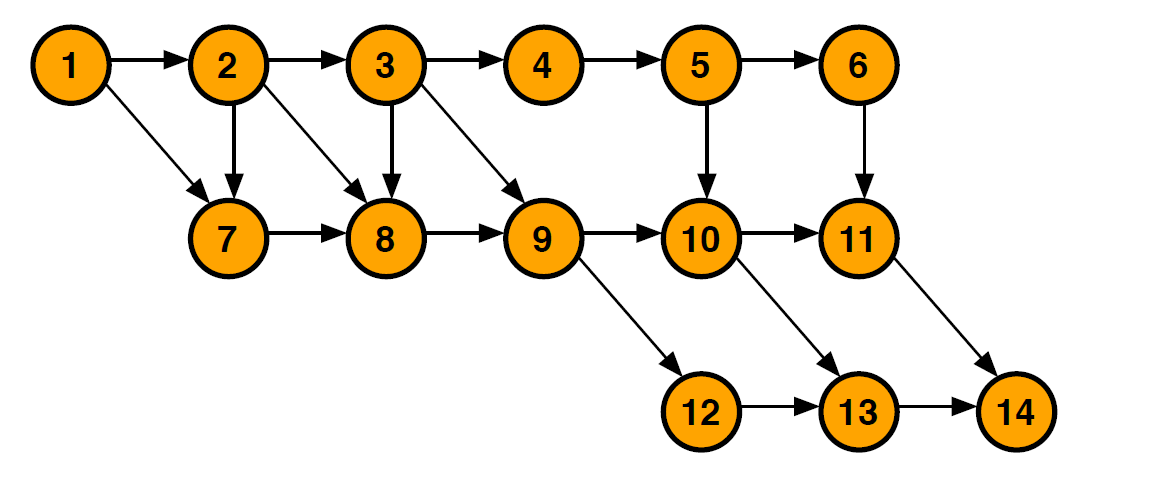
\includegraphics[scale=0.4]{graph.png}
        \caption{Thormund's Network}
        \label{fig:my_label}
    \end{figure}
    
    \pagebreak
    
	\item (20 points) As a new event in the Triwizard Tournament, students must compete in pairs in the following game. An even number $n$ of magical items are laid out in a row, with the $i$-th item having a value of $v(i)$ in Knuts for each $i=1,2,\dotsc,n$. The players alternate turns, and on each turn, the player may choose either the first item or the last item remaining in the row, then remove it from the row and add it to their pile. The player with the highest-valued pile at the end wins. (The value of a player's pile at the end is simply the sum of the value of the items in the pile.) We will use dynamic programming to help us analyze this game.
	
	\begin{enumerate}
	\item For a given vector $v$ of values, let $F(i,j)$ denote the maximum value that the first player can definitely achieve using the values $v[i], \dotsc, v[j]$---this means a \emph{tight}, \emph{exact} upper bound, an amount which the first player cannot beat, but that the first player can in fact achieve if he/she plays optimally. Write down a recurrence relation for $F(i,j)$ and prove that it is correct. Be sure to include a base case!  You can assume that this problem has optimal substructure.
	
	\item Based on your recurrence from part (a), describe a dynamic programming table and the order in which it should be filled in.
	
	\item Write pseudo-code for the dynamic programming solution you described in part (b) and analyze its run-time.
	
	\end{enumerate}

\end{enumerate}
\end{document}


